La figura \ref{fig:gantt_real} muestra el diagrama de Gantt con la planificación real del proyecto.  La planificación real responde al ritmo real con el que se ha desarrollado el proyecto.  Al igual que sucedió con la planificación inicial, cabe destacar que una vez por semana se ha realizado una reunión de seguimiento por parte del equipo de desarrollo.\\
La planificación real ha resultado en unas 970 horas de trabajo.

Las diferencias entre la planificación inicial y real son varias y se explicarán con detalle en la siguiente sección de éste capítulo.

\begin{figure}[h]
	\centering
	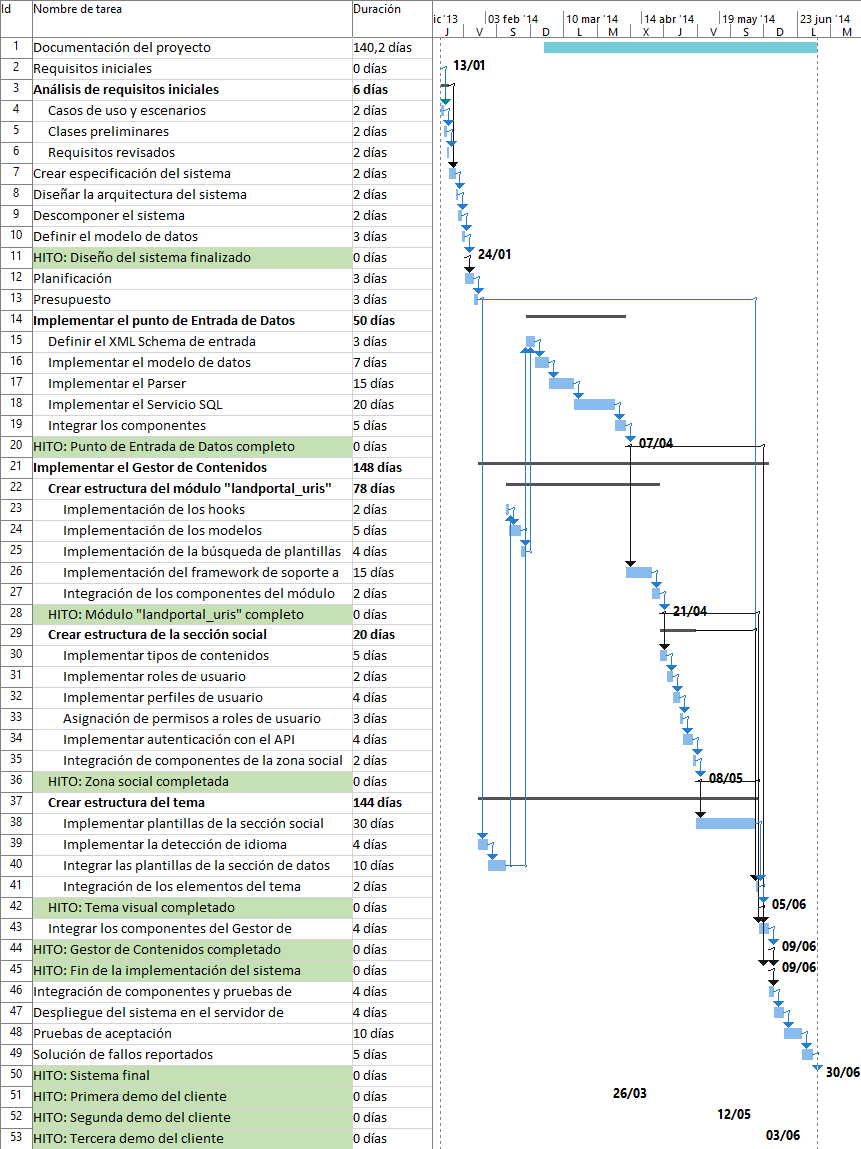
\includegraphics[width=\textwidth]{planificacion/real}
	\caption{Diagrama de Gantt con la planificación real del proyecto}
	\label{fig:gantt_real}
\end{figure}